\chapter{Kapitel 3}

Der Speicher ist, neben der CPU, eines der wichtigsten Betriebsmittel in einem Rechnersystem. Eine Kernaussage, bekannt als Parkinsons Gesetz angewandt auf Speicher, lautet: „Die Programme expandieren, um den zugänglichen Speicher, der sie enthält, auszufüllen.". Der Teil des Betriebssystems, der die Speicherhierarchie verwaltet, wird als \textbf{Speicherverwaltung} (Memory Manager) bezeichnet.

\section{Systeme ohne Speicherverwaltung}

Frühe Computersysteme, wie Großrechner vor 1960 und PCs vor 1980, kamen ohne Speicherabstraktion aus. Das bedeutet, dass Programme direkt auf den physikalischen Speicher zugegriffen haben. Ein Mehrprogrammbetrieb war unter diesen Umständen nicht möglich.

Um dennoch mehrere Programme ausführen zu können, wurden zwei grundlegende Techniken entwickelt:

\subsection{Swapping}
Beim Swapping wird der gesamte Speicherinhalt auf eine Platte ausgelagert (geswappt), um Platz für ein neues Programm zu schaffen. Nachdem das neue Programm abgearbeitet wurde, kann das nächste geladen werden.

\subsection{Statische Relokation}
Hierbei werden die Adressen eines Programms beim Laden in den Speicher angepasst. Das Betriebssystem addiert eine Startadresse auf alle Speicheradressen des Programms. Eine Herausforderung dabei ist die Unterscheidung zwischen Adressen und Konstanten, was den Ladevorgang verlangsamt.

\section{Speicherabstraktion: Der Adressraum}

Die Speicherabstraktion löst die Probleme der direkten Adressierung durch die Einführung von Adressräumen. Der \textbf{Adressraum} ist die Menge aller Adressen, die ein Prozess zur Adressierung des Speichers nutzen kann. Jeder Prozess erhält seinen eigenen, von anderen Prozessen getrennten (disjunkten) Adressraum.

\subsection{Relokation und Schutz}
Die Speicherabstraktion ermöglicht es, verschiedene Prozesse an unterschiedliche Stellen im physikalischen Speicher zu laden (Relokation) und sie voreinander zu schützen. Eine Hardware-Lösung hierfür verwendet ein \textbf{Basisregister} und ein \textbf{Limitregister}.
\begin{itemize}
    \item Das \textbf{Basisregister} wird bei einem Prozesswechsel mit der Startadresse des Prozesses im physikalischen Speicher geladen.
    \item Das \textbf{Limitregister} enthält die Länge des für den Prozess reservierten Speicherbereichs (Partition).
\end{itemize}
Bei jedem Speicherzugriff wird die vom Prozess generierte Adresse zunächst mit dem Limitregister verglichen. Ist die Adresse größer oder gleich dem Limit, wird ein Fehler ausgelöst (Schutzverletzung). Andernfalls wird die Adresse zum Inhalt des Basisregisters addiert, um die physikalische Adresse zu erhalten. Der Nachteil ist, dass bei jedem Speicherzugriff eine Addition und ein Vergleich notwendig sind, wobei die Addition als teuer (zeitaufwendig) gilt.

\subsection{Swapping mit Speicherabstraktion}
In modernen Mehrbenutzersystemen ist die Anzahl der Prozesse oft größer als der verfügbare physikalische Speicher. Swapping ist hier eine gängige Strategie:
\begin{itemize}
    \item Prozesse werden vollständig in den Speicher geladen, laufen für eine bestimmte Zeit und werden dann wieder in den Hintergrundspeicher ausgelagert.
    \item Dies führt zur \textbf{Fragmentierung} des Speichers, es entstehen Lücken. Diese Lücken zu schließen (Speicherverdichtung) ist sehr zeitaufwendig. Eine 16-GB-Maschine, die 8 Bytes in 8 ns kopiert, benötigt für die Verdichtung ca. 16 Sekunden.
    \item Da Prozesse oft wachsen, ist es sinnvoll, bei der Einlagerung etwas mehr Speicher zu reservieren. Beim Auslagern wird nur der tatsächlich belegte Speicher auf die Platte geschrieben.
\end{itemize}

\subsection{Verwaltung von freiem Speicher}
Zur Verwaltung von freiem Speicher gibt es hauptsächlich zwei Methoden:

\subsubsection{Speicherverwaltung mit Bitmaps}
Der Speicher wird in \textbf{Allokationseinheiten (AE)} unterteilt. Für jede AE gibt es ein Bit in einer Bitmap (0 = frei, 1 = belegt).
\begin{itemize}
    \item \textbf{Vorteil:} Einfachheit.
    \item \textbf{Nachteil:} Die Größe der Bitmap hängt von der Größe der AE ab. Kleine AEs führen zu großen Bitmaps, während große AEs zu interner Fragmentierung führen (eine AE ist im Mittel nur zur Hälfte belegt).
\end{itemize}

\subsubsection{Speicherverwaltung mit verketteter Liste}
Freier und belegter Speicher wird in einer nach Adressen sortierten, verketteten Liste verwaltet. Jeder Eintrag in der Liste repräsentiert entweder einen Prozess (P) oder ein Loch (L) und enthält die Startadresse, die Länge und einen Zeiger auf den nächsten Eintrag. Wenn ein Prozess terminiert, werden angrenzende Löcher verschmolzen.

\paragraph{Algorithmen zur Speicherallozierung:}
\begin{itemize}
    \item \textbf{First Fit:} Wählt das erste passende Loch in der Liste. Der Algorithmus ist schnell.
    \item \textbf{Next Fit:} Wie First Fit, aber die Suche beginnt bei der letzten gefundenen Position.
    \item \textbf{Best Fit:} Durchsucht die gesamte Liste und wählt das kleinste passende Loch. Führt zu viel ungenutztem, kleinen Speicherfragmenten.
    \item \textbf{Worst Fit:} Wählt das größte verfügbare Loch, was ebenfalls zu Speicherverschwendung führt.
    \item \textbf{Quick Fit:} Verwaltet separate Listen für häufig nachgefragte Lochgrößen (z.B. 4K, 8K). Dies ist sehr schnell, aber das Verschmelzen von Lücken ist aufwändig.
\end{itemize}

\subsection{Speicherverwaltung mit dem Buddy-System}
Dieses System nutzt die binäre Adressierung von Rechnern.
\begin{itemize}
    \item Es werden Listen von freien Blöcken in Zweierpotenzgrößen (1, 2, 4, 8, ... KB) verwaltet.
    \item Bei einer Anforderung für einen Block der Größe $k$ wird eine Liste mit Blöcken der Größe $2^m$ gesucht, wobei $2^{m-1} < k \le 2^m$.
    \item Ist kein Block der passenden Größe frei, wird ein größerer Block rekursiv halbiert ("Buddies"), bis ein passender Block entsteht.
    \item \textbf{Nachteil:} Hohe interne Fragmentierung, da immer auf die nächste Zweierpotenz aufgerundet wird.
\end{itemize}

\section{Virtueller Speicher (Extrem prüfungsrelevant)}

Beispielsweise Filme sind zu groß, um in die meisten Haupspeicher geladen zu werden. Dennoch ist es möglich, Filme auf Computern zu gucken. Programme im allgemeinen sind zu groß für den Speicher. Aufgrunddessen müssen zur Laufzeit Programme (zumindest Teilweise) ein- und Ausgelagert werden. Zur Laufzeit wird dann entschieden, welches Programm und welche Teile des Programms in den Hauptspeicher geladen werden soll. 

Swapping ist hier eine mögliche lösung, jedoch keine gute, da es sehr lange dauert, gesammte Prozesse samt ihres Contextes in den Hauptspeicher zu swappen.

\subsection{Grundidee}

Der Haupspeicher wird in einzelne Teile aufgeteilt (sog. Seiten). Jede Seite ist ein aneinander angrenzender Bereich von Adressen. Das Betriebssystem hält nur die aktuell relevanten Seiten im Hauptspeicher, alle anderen Seiten sind im Massenspeicher gespeichert. Bei Filmen werden also beispielsweise nur die nächsten 10 Frames im Hauptspeicher geladen. Damit muss nur eine halbe Sekunde des Films anstelle von mehreren Stunden langen Film im Hauptspeicher gespeichert sein.

Seiten, welche im Hauptspeicher sind, nennt man PageFrames. Andere Seiten werden Virtuelle Seiten genannt. Wird auf eine Virtuelle Seite zugegriffen, erfolgt ein Seitenfehler. Das Betriebssystem muss nun dafür sorgen, dass die angeforderte Seite in den Hauptspeicher gelangt. Hierbei kann es passieren, dass der Hauptspeicher nicht genug Platz für die neue Seite hat. Deshalb muss mittels eines Seitenersetzungsalgorithmuses eine alte Seite aus den Hauptspeicher gelöscht werden.

Sobald Virtuelle Seite in Hauptspeicher geladen ist, muss der ausgeführte Befehl restauriert werden, sodass der Befehl noch einmal ausgeführt werden kann.

\subsection{Paging}

Jeder Rechner hat eine Menge von virtuellen Speicheradressen. 

MOVE REG, 1000

kopiert die Speicherstelle 1000 in das Register oder umgekehrt.

die von Programmen generierten Adressen werden \textit{virtuelle Adressen} genannt. Alle Programme bilden den virtuellen Adressraum. Der Virtuelle Speicher ist meist um einen faktor 1000000 größer als der tatsächliche Hauptspeicher. Um sicherzustellen, wo die Virtuellen Adressen im Hauptspeicher abgelegt sind, wird die gls{MMU} benötigt.

\subsection{Seitentabellen}

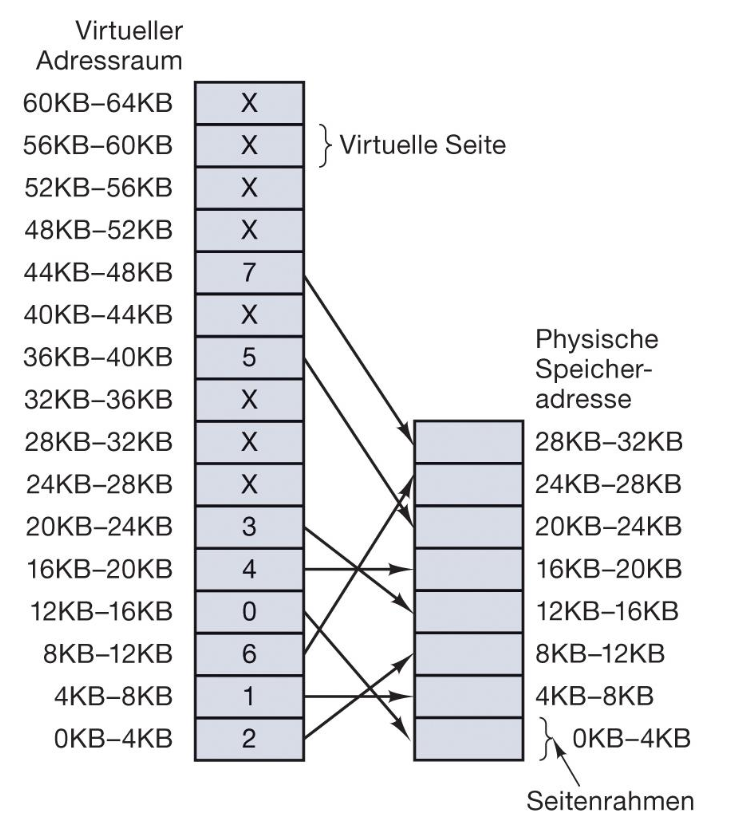
\includegraphics[width=\textwidth]{virtuelle_adressen.png}

Die Virtuellen Adressen 0KB-4KB ist im Seitenrahmen 2, die Virtuellen Adressen 4KB - 8KB ist im Seitenrahmen 1 usw. Virtuelle Adressen wie beispielsweise 24KB - 28KB sind gar nicht im Hauptspeicher. Wenn auf diese zugegriffen werden soll, müssen diese in den Hauptspeicher geladen werden.

Der Virtuelle Adressraum wird in Seiten gleicher Größe eingeteilt (512 Byte - 1GB üblich). Seiten und Seitenrahmens ind idr. gleich groß. Zwischen RAM und Festplatte werden immer nur komplette Seiten übertragen. Um zu prüfen, ob eine Virtuelle Seite im Speicher ist, wird das Present/absent- Bit überprüft.

\subsection{Pagefault (Seitenfehler)}

Wenn auf eine nicht vorhandene Seite zugegriffen wird, ist das Present-Bit = 0. Die MMU muss nun per Interrupt sicherstellen, dass die benötigte Seite in den Hauptspeicher geladen wird. Hierfür überprüft die MMU zunächst, ob noch freier Platz zur verfügung steht. Wenn nicht wird ein Seitenersetz\-ungsalgorithmus aufgerufen, um eine Seite zu ersetzen. Hierbei ist es möglich, dass diese Seite bearbeitet wurde. Wenn eine Seite im Hauptspeicher bearbeitet wurde, muss sie zunächst zurück in den Massenspeicher geschrieben werden, um Datenverlust zu verhindern. Auch das Present- und Absent bit muss von der MMU gesetzt werden. Der BEfehl, der den Pagefault ausgelöst hat, wird wiederholt.

\subsubsection{Interne Operationen der MMU}

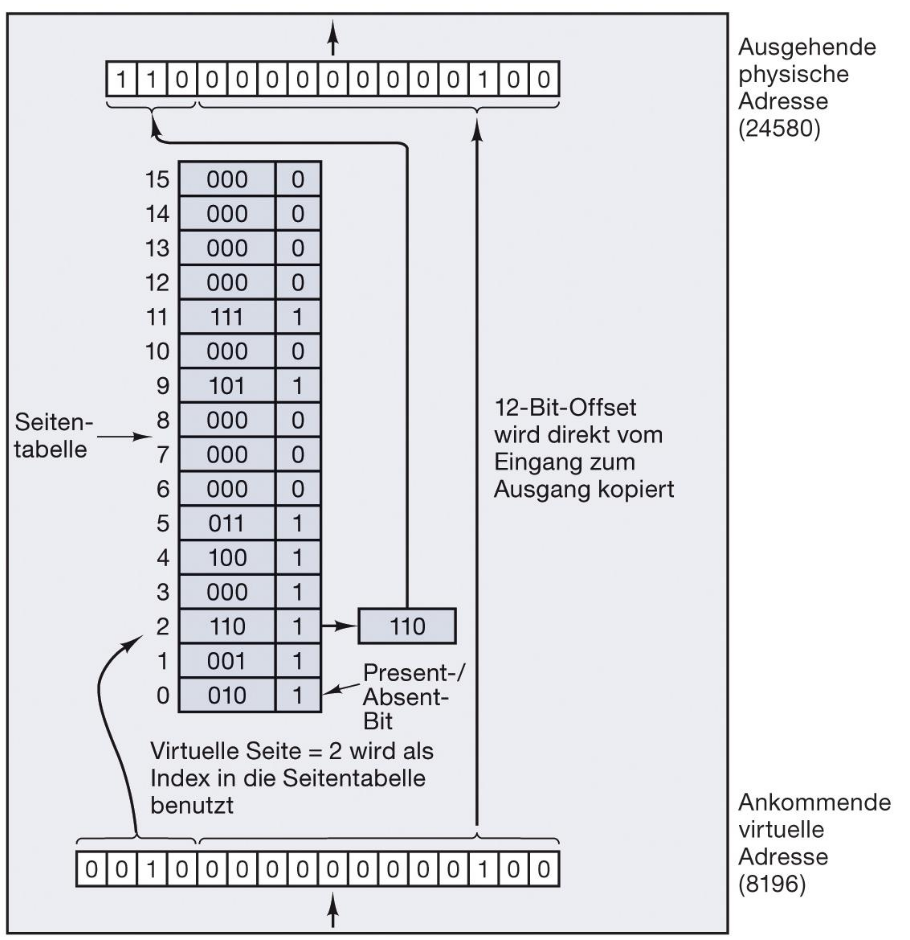
\includegraphics[width=\textwidth]{interne_operationen_der_mmu.png}

Unten steht Virtuelle Seitennummer. Die vorderen vier Bit werden als Index für Seitentabelle verwendet. hier 0010 steht für Eintrag 2 an Seitentabelle. Present/Absent bit ist hier gesetzt, sprich die Seite ist im Hauptspeicher vorhanden. Die tatsächliche Adresse wird dann als Prefix an die Tatsächliche Phsysikalische Adresse gesetzt. Dies funktioniert, da mit zweierpotenzen gerechnet werden. Die Seitennummer kann einfach mit der Adresse innerhalb der Seite Konkartiniert werden.

Die Seitentabelle dient als Abbildung einer Virtuellen adresse auf Physikalischen Seitenrahmen. 

\subsection{Einträge der Seitentabelle}

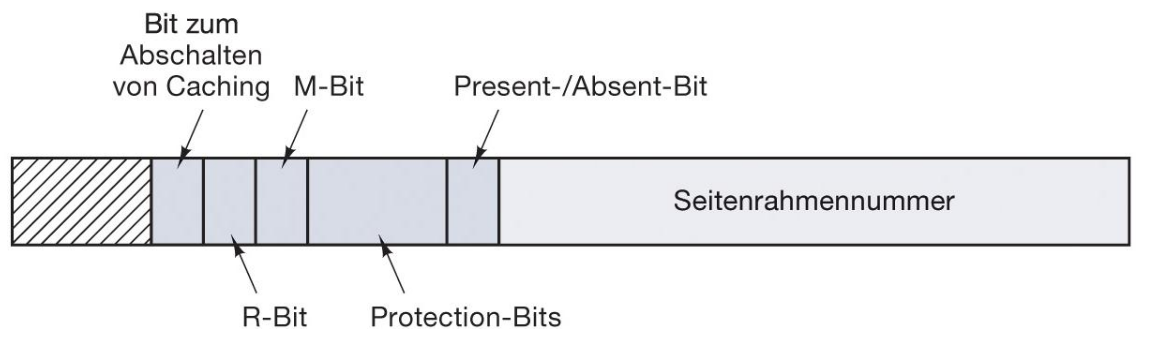
\includegraphics[width=\textwidth]{seitentabelleneintrag.png}

In der Seitentabelle steht, ob Cashing eingeschalten oder abgeschalten ist. Wenn häufig auf eine Seite zugegriffen wird, kann sie gecashed werden. Hier kann sich der Inhalt der Seite im Massenspeicher von der im Cash unterscheiden. Das \textit{R-Bit} (Reference Bit) sagt aus, ob in letzter Zeit auf diese Seite zugegriffen wurde. Das \textit{M-Bit} (Modify Bit oder Dirty Bit) sagt aus, ob die Seite modifiziert wurde. Wenn die Seite nicht modifiziert wurde, muss sie nicht zurück in den Massenspeicher zurückgeschrieben werden, da die Seiten im Haupt- und Massenspeicher identisch sind. Die Protection-Bits (read, write, execute) sagen aus, ob und wer die Seite ausführen, lesen und schreiben darf.

\subsection{Beschleunigung des Paging}

Die umrechnung von virtuellen zu Phsyikalischen Adressen muss sehr schnell erfolgen. Hierfür könnte mit registern gearbeitet werden, dies funktioniert in der realität allerdings nicht, da Seitentabellen sehr groß werden können (bei 64Bit rechner und 4k großen Seiten ist Tabelle $2^{54}$ Byte lang. das sind 52 Petabyte!).

Eine andere lösung wäre, dass sich die Seite komplett im Arbeitsspeicher befindet. Hier könnte ein Register auf den Anfang der Seitentabelle zeigen. Dann müsste allerdings bei jeder Speicherreferenz auf diese Seitentabelle zugegriffen werden, wodurch jeder \texttt{I/O} Zugriff sehr viel langsamer wird.

\subsection{TLB - Translation Lookaside Buffer}

Bisher ist davon ausgegangen, dass Seitentabellen im Speicher sind. Dies hat jedoch die oben genannten nachteile. Man Beobachtete, dass die meisten Programme eine große Anzahl von Referenzen auf eine kleine Anzahl von Seiten beschränken. Dies bedeutet, dass eine kleine Anzahl an Seiten häufiger benötigt werden. Ein Videoplayer wird beispielsweise die meiste Zeit für das Darstellen des Videos verhältnismäßig wenige Seiten benötigen. Am Anfang wird er jedoch viele Seiten benötigen. 

Es werden innerhalb der MMU eine kleine Anzahl an Seiten zwischengespeichert. Die Zuordnung der virtuellen Seiten wird in einem sog. \texttt{Translation Lookaside Buffer} gespeichert. Dieser ist extrem schnell, aber auch extrem teuer.

\subsubsection{Aufbau}

Der \texttt{TLB} Befindet sich innerhalb der MMU. Er verwaltet nur eine kleine Anzahl an einträgen und kann Hardwarebasiert innerhalb eines Taktes die gesammte gespeicherte Seitentabelle durchsuchen. Wenn eine Seitentabelle nicht innerhalb des \texttt{TLB} gefunden wird, wird diese aus dem Hauptspeicher geholt und in den \texttt{TLB} eingelagert.

\subsubsection{Arbeitsweise des \texttt{TLB}}

\begin{itemize}
    \item Virtuelle Adresse wird an MMU gesendet
    \item Hardware durchsucht parallel alle Einträge des \texttt{TLB} nach der Virtuellen Adresse
    \item Bei hit und keine Schutzcodeverletzung wird Seitenrahmennummer aus \texttt{TLB} verwendet.
    \item Bei hit und Schutzcodeverletzung kommt Schutzfehler-Außnahme
    \item bei Miss durchsucht MMU die Seitentabelle.
    \item Eintrag aus dem \texttt{TLB} wird durch den gefundenen Ersetzt
\end{itemize}

\subsubsection{Erhöhung der hit-rate}

Trefferrate ist der Bruchteil der Speicherreferenzen mithilfe des \texttt{TLB} bedinet werden kann. Jehör die Hit-rate ist, desto besser ist die Performance. Die Performance hängt von drei Faktoren ab:

\begin{enumerate}
    \item Zugriffszeit auf Seitentabelle
    \item Zugriffszeit auf \texttt{TLB}
    \item Trefferrate
\end{enumerate}

Die Trefferrate hängt also von der mittleren Anzahl der Seiten und der größe des \texttt{TLB} ab. Die Performance kann weiterhin erhöht werden, indem der \texttt{TLB} Prefetched wird.

\subsubsection*{Cashing von \texttt{TLB} Einträgen}

Der \texttt{TLB} kann auch gecahsed werden.

\subsection{Seitentabellen für große Speicherbreite}

Seitentabellen sind heutzutage sehr sehr groß. Die gesammte Seitentabelle kann rein physikalisch nicht gesammt im Hauptspeicher gespeichert sein. Aus diesen grund gibt es \textit{Mehrstufiges Paging}. Die Virtuelle Adresse wird in mehrere Tabellen aufgeteilt.

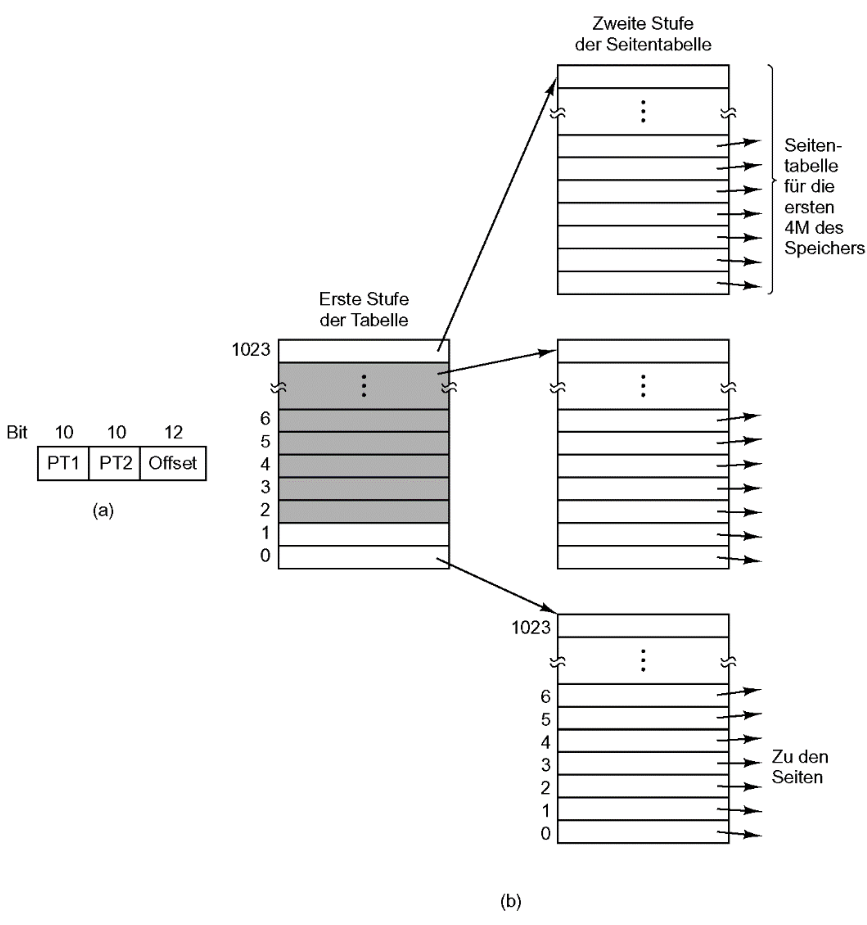
\includegraphics[width=\textwidth]{zweistufige_seitentabelle.png}

Anstelle nur eines Bit für die Seitentabelle teilt man die Seitentabellenadresse in mehere Bit ein. so steht ein Bit für die Seitentabelle, in welcher weitere Seitentabellen sind. Der zweite Bit steht dann für die über die Seitentabelle gefundene Seitentabelle, in welcher dann der tatsächliche Seitenrahmen steht.

In der realität wird dies nicht nur mit zweistufigen Paging, sondern mit mehrstufigen Paging durchgeführt. Beispielsweise besitzt der \texttt{80386} 4GB adressierbaren Speicher. Hier wird zweistufiges Paging verwendet. Der Pentium Pro hingegen hatte auch 4GB Adressierbaren Speicher, jedoch hat dieser 4 Stufiges Paging. Die X86-Familie mit 64 Bit besitzt 256TB adressierbaren Speicher addressierbar und 4  Stufiges Paging.

Mehrstufiges Paging erhöht den Overhead des Speicherzugriffs. Beispielsweise ist 4-Stufiges Paging 5 mal langsamer als Physikalische Adressen, da auf 4 Seitentabellen und dann noch auf die Physikalische Adresse zugegriffen werden muss.

\subsubsection{Invertierte Seitentabellen}

Alternativ zu den ständig zunehmenden Stufen der Paging-Hierarchie wird ein Eintrag pro Seitenrahmen zugewiesen. 

\subsubsection*{Vorteil}

Es wird viel Speicher gespaart, wenn Physikalischer Speicher wesentlich kleiner als Virtueller Speicher ist. -> Ist heutzugage immer der fehleranfällig

\subsubsection*{Nachteile}

Wenn Prozess n auf Seite p zugreifen will, so muss er bei \textbf{jedem} Speicherzugriff die gesamte Seitentabelle nach dem paar \textit{(n,p)} durchsuchen -> sehr sehr langsam. Der \texttt{TLB} hilft zwar, allerdings bei einem TLB Fehler erfolgt das suchen der Seitentabelle per Software. Schnellere Suche ermöglichen Hashtabellen mit den virtuellen Adressen als Hashwert. 

\subsubsection*{Vergleich zwischen herkömmlicher und invertierter Seitentabelle}

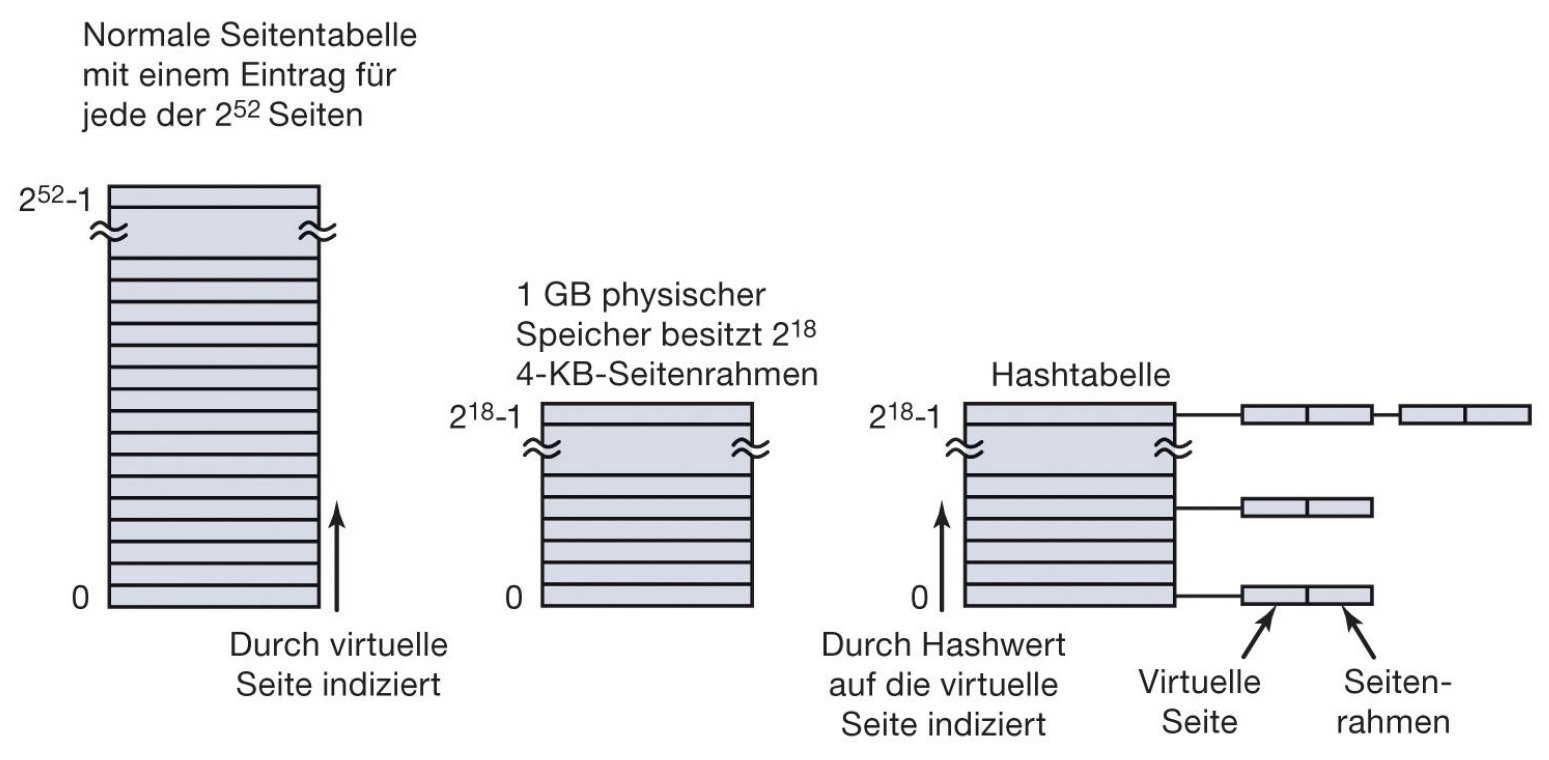
\includegraphics[width=\textwidth]{vergleich_seitentabellen_invertierten_seitentabellen.png}

\section{Seitenerzetzungsalgorithmen}

Durch Seitenersetzungsalgorithmen sollen zu häufige Seitenfehler vermieden werden. Die Fragestellung ist, welche seite am besten aus dem Hauptspeicher geholt wird. Hier sollte am besten eine Seite ausgelagert werden, welche in der Zukunft nicht so häufig verwendet wird. 

\subsection{Optimaler Seitenersetzungsalgorithmus}

Der Optimale Seitenersetzungsalgorithmus nimmt die Seite, die erst am weitesten in der Zukunft benötigt wird, und wirft sie aus den Speicher. Dies ist selbstverständlich nicht umsetzbar, jedoch ist der Optimale Seitenersetzungsalgorithmus sehr sinnvoll für Vergleichszwecke.

\subsection{Not-Recently-Used-Algorithmus (NRU)}

Es gibt zwei Bits im Rechner, die die Nutzung von Seiten protokollieren: das R- und M-Bit. Das R-Bit wird gesetzt, wenn die Seite referenziert wurde. Das M-Bit wird gesetzt, wenn eine Seite bearbeitet wird. Beide Bits bleiben gesetzt, bis das Betriebssystem diese zurücksetzt. Die Bits werden regelmäßig zurückgesetzt.

Bei jedem Timerinterrutp wird das R-Bit zurückgesetzt. Bei Seitenfehler werden alle Seiten in vier Klassen klassiviziert

\begin{enumerate}
    \item Klasse 0: Nicht referenziert, nicht Modifiziert (guter Kanidat zum ersetzen)
    \item Klasse 1: nicht referenziert, modifiziert
    \item Klasse 2: referenziert, nicht modifiziert
    \item Klasse 3: referenziert, modifiziert
\end{enumerate}

NRU entfernt zufällig eine Seite aus der Kleinstnummerierten, nicht leeren Klasse. Dieser Algo ist sehr einfach implementiert. Die Leistung ist zwar nicht Optimal, aber oft ausreichend.

\subsection{First-In-First-Out-Algorithmus FIFO}

Die älteste Seite befindet sich am Ende der Liste. die Neuste am Anfang. Es wird immer die älteste Seite ausgeworfen.

\subsection{Second-Chance-Algorithmus}

Der Second-Chance-Algorithmus ist eine Modifikation des FIFO-Algorithmus. Wenn die älteste Seite den R-Bit = 0 ist, wird sie entfernt. Wenn das R-Bit = 1 ist, wird die Seite nach vorne gestellt. Dies geschiet so lange, bis eine Seite gefunden wurde, bei welcher das R-Bit = 0 ist. Wenn keine Seite gefunden wird, wird die Älteste Seite entfernt.

\subsection{Clock-Algorithmus}

Der Clock-Algorithmus ist eine Variation des Second-Chance-Algorithmus. Die Seiten sind als Kreis dagestellt. Ein Zeiger zeigt auf die Älteste Seite. Wenn ein Seitenfehler auftritt, wird die Seite, auf die der Zeiger zeigt analysiert. Wenn R-Bit = 0 ist, wird die Seite ausgelagert. Wenn das R-Bit = 1 ist, wird R-Bit auf 0 gesetzt und der Zeiger rückt weiter.

\subsection{Least-Recently-Used-Algorithmus (LRU)}

Der Least-Recently-Used-Algirhtmus bildet eine Approximation des Optimalen Algorithmuses ab. Es werden die Seiten entfernt, die am längsten unbenutzt sind. Die Listen werden nach jedem Zugriff aktualisiert. Diese Liste zu pflegen sit sehr aufwändig, weshalb es mögliche umsetzung in Hardware gibt. Es wird ein Hardware 64Bit zähler bei jedem Zugriff inkrementiert. Die Seite mit dem niedrigsten Zählerstand wird dann ausgeworfen. Wenn eine Seite in der Vergangenheit sehr häufig benutzt wurde, bleiben unter Umständen für immer im Hauptspeicher.

\subsection{Not-Frequently-Used-Algorithmus (NFU)}

Software Variation des LRU. Es wird Periodisch das R-Bit auf einen Zähler addiert. Die Seite mit den kleinsten Zählerstand wird dann entfernt. Auch hier ist das Problem, dass hohe Zählerstände nicht vergessen werden.

\subsection{Aging-Algorithmus}

Modifikation des NFU. Die Zähler werden alle ein Bit nach rechts geschoben, bevor das R-Bit addiert wird. Das R-Bit wird auf das am weitesten Links stehende Bit addiert.

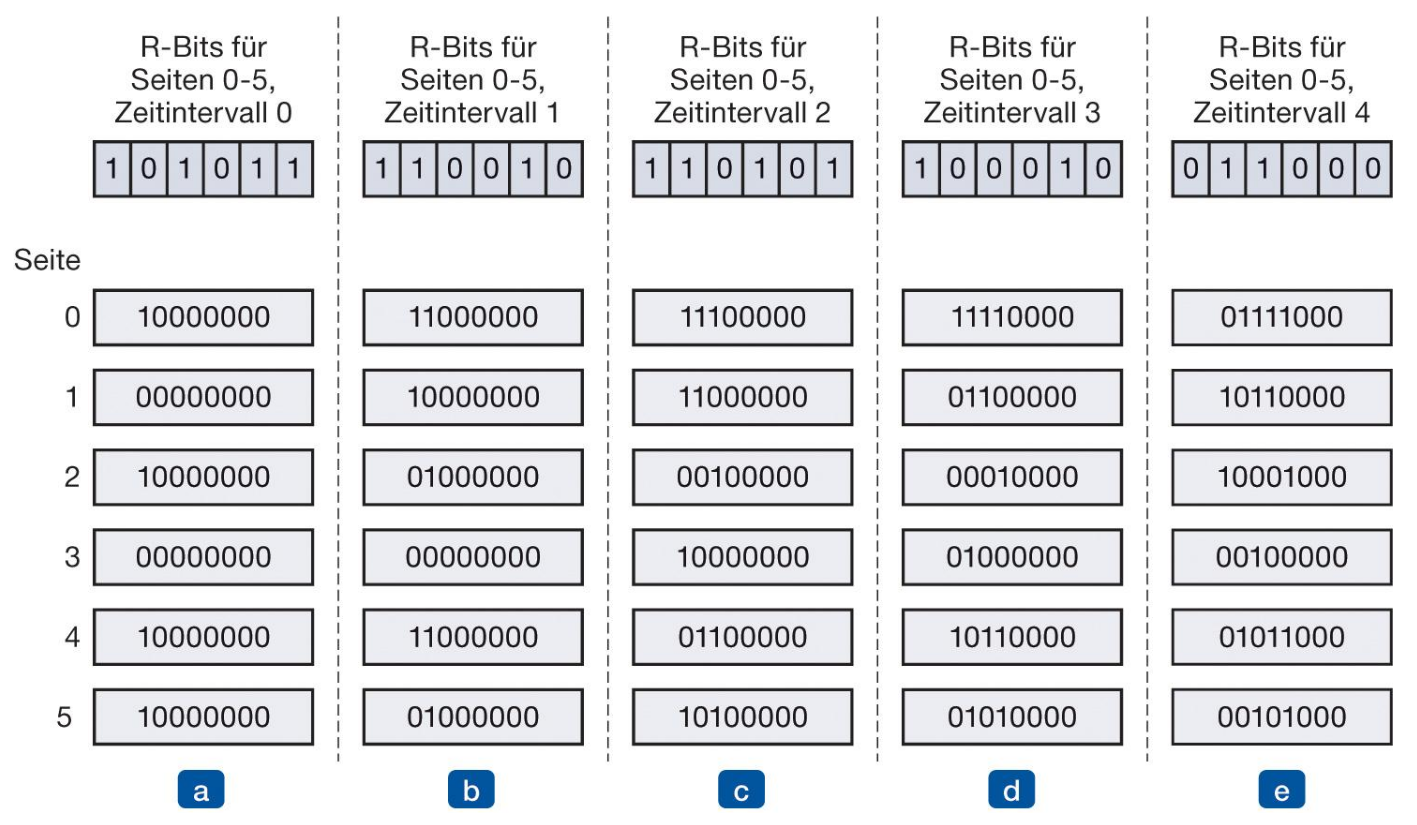
\includegraphics[width=\textwidth]{aging.png}

\subsection{Working-Set-Algorithmus}

Reinste form des Paging. Bei Prozessstart ist keine Seite im Speicher. Überzeit kommen mehr und mehr Seiten in den Hauptspeicher. Die Lokalitätseigenschaft besagt, dass wärend der Ausführung eines Programms nur ein Bruchteil seiner Seiten benötigt werden. Der Arbeitsbereich beschreibt die Menge der Seiten, die ein Prozess zur ausführung benötigt. Ist der gesammte Arbeitsbereich im Speicher, so entstehen keine Seitenfehler.

Wenn Prozesse vollständig aus den Arbeitsspeicher verdrängt wurden, werden viele Seitenfehler auftauchen. Dies kann den Prozess sehr stark verlangsamen, um den Faktor 1 bis 10 Mio. Dies wird Thrashing oder Seitenflattern genannt. Das Anlaufverhalten sollte also verbessert werden.

Es wird versucht, den gesammten Arbeitsbereich eines Prozesses in den Speicher zu bekommen. 

Idee für die Umsetzung ist also dass der Arbeitsbereich identifiziert werden muss. Dies funktionier auch mit Seitenersetzungsalgorithmen. Es werden nicht nur die letzten k-Speicherzugriffe betrachtet, sondern die Ausführungszeit des Prozesses. Es wird eine Virtuelle Zeit eingeführt, welche ein Prozess zum start initialisiert hat. Der Arbeitsbereich eines Prozesses sind die Seiten, die ein Prozess in den letzten $\tau$ Sekunden benutzr hat. Bei einem Seitenfehler werden die Seiten ausgelagert, die nicht länger zu dem Arbeitsbereich gehören und das R-Bit 0 ist. 

\subsection{Working-Set-Clock-Algorithmus}

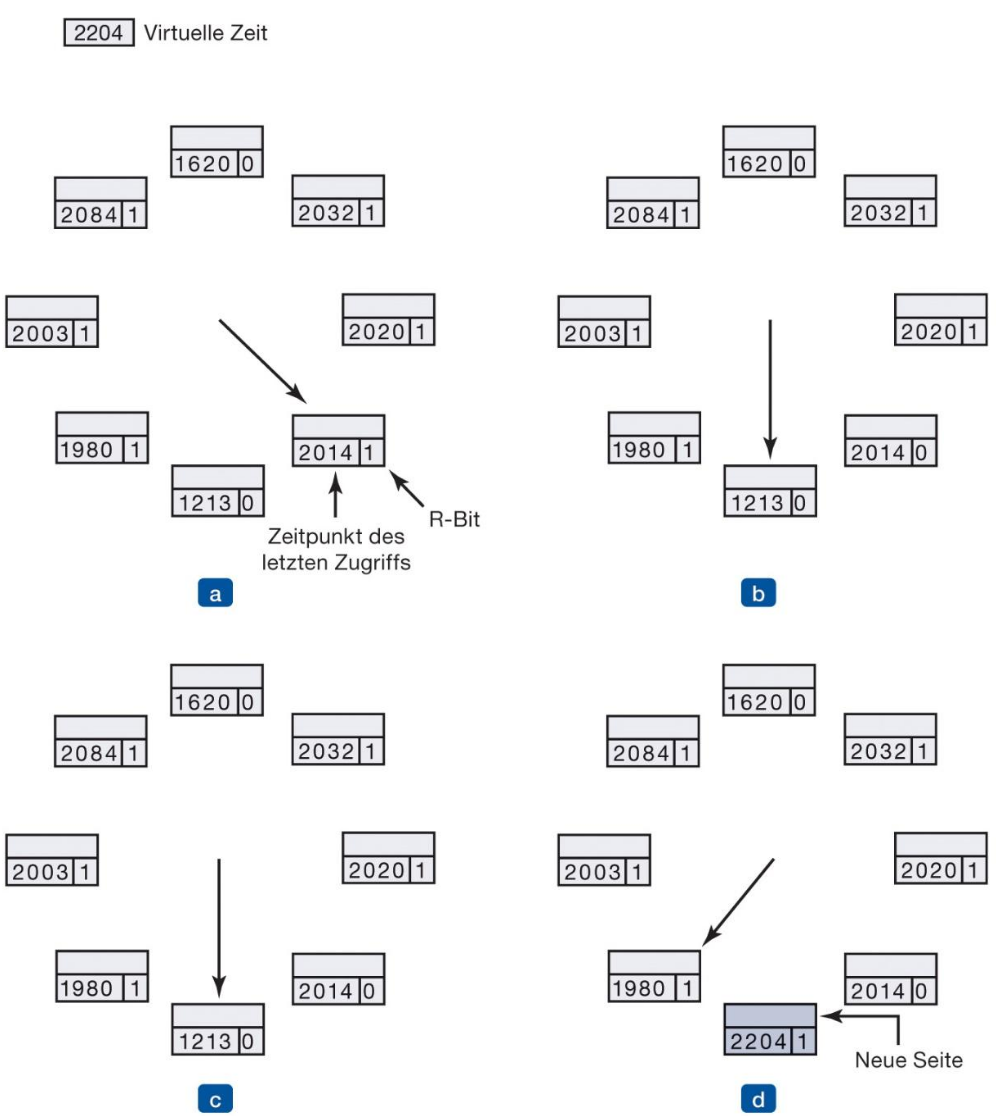
\includegraphics[width=\textwidth]{wsclock.png}

Wenn Seite gefunden wird, die außerhalb des Workingsets ist, wird so lange weitergesucht, bis Seite rausgeschrieben wird, die ersetzt werden kann.

\section{Entwurfskriterien fürs Paging}

Beim einführen von Paging gibt es mehrere dinge die betrachtet werden müssen.

\subsection{Pagefaultfrequency Algorithmus}

Der Pagefaultfrequency Algorithmus (PFF-Algorithmus) versucht, die Seitenfehler pro Sekunde zwischen einem Minimum und Maximum zu behalten. 

\subsection{Lastkontrolle}

Trotz gutem Seitenersetzungsalgorithmus und optimaler globaler SPeicherzuteilung können viele Seitenfehler auftreten. Der Arbeitsbereich aller Prozesse ist also grö0er als der verfügbare Arbeitsspeicher. Um dies zu verhindern, kann ein gesammter Prozess ausgelagert werden, sodass Seitenflattern verhindert wird.

\subsection{Seitengröße}

Die Seitengröße sollte nicht zufällig gewählt werden. Bei kleinen Seiten gibt es eine sehr kleine interne Fragmentierung, was zu sehr guter Auslastung des Arbeitsspeichers führt. Allerdings wird die Seitentabelle auch sehr groß sein. Bei einer sehr großen Seitengröße ist die Seitentabelle zwar sehr klein und die Seiten können sehr schnell vom Massenspeicher geholt werden, allerdings ist die interne fragmentierung sehr groß wodurch der Arbeitsspeicher nur sehr schlecht genutzt wird.

\subsubsection*{Mathematische Analyse}

\begin{align*}
    Overhead(p) = \frac{s \cdot e}{p} + \frac{p}{2} \\
    Overhead'(p) = \frac{- s \cdot e}{p^2} + \frac{1}{2} = 0 \Rightarrow p_{opt} = \sqrt{2 \cdot s \cdot e}
\end{align*}

Für s = 1MB und e = 8 Byte ist also die Optimale Seitengröße 4KB. In heutigen Rechnern ist eine Seitengröße von 512 Byte bis 64KB typisch.